\section{Budowa pojazdu - założenia i testy}
    Inspiracją do stworzenia poniższego projektu, były samochody autonomiczne, które najczęściej są pojazdami dwuosiowymi, o jednej osi skrętnej i jednej osi napędzającej.
    Obie osie, nie będą połączone ze sobą, co pozwoli na niezależne sterowanie nimi.
    W projekcie zostaną użyte dwa silniki prądu stałego wybrane w rozdziale \ref{sec:engines}.
    Silniki zostały podłączone bezpośredni do kół w osi tylnej.
    \subsection{Przednia oś}
        Przednia oś, została połączona układem kierowniczym, opartym na serwomechaniźmie.
        Na rysunku \ref{fig:frontAxis_model} przedstawiono model układu kierowniczego zaprojektowanego przez autorów.

        \begin{figure}[!ht]
            \centering
            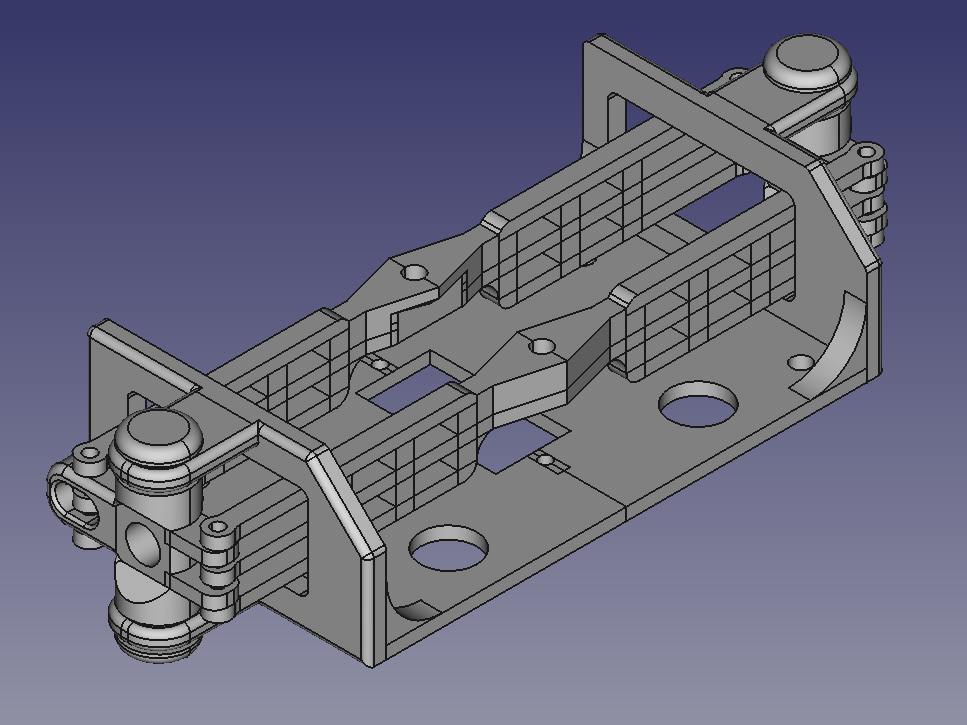
\includegraphics[width=0.7\textwidth]{FronAxis_example.png}
            \caption{Przykładowy układ kierowniczy zaprojektowany w narzędziu FreeCAD}
            \label{fig:frontAxis_model}
        \end{figure}
        Układ został skręcania, został zaprojektowany w taki sposób aby ramiona skrótów oraz ramie serwomechanizmu były takiej samej długości.
        Dzięki temu, kąt ustawienia serwomechanizmu, odpowiada kątowi skrętu kół.
        Natomiast dużą wadą takiego układu, jest brak możliwości odczynia aktualnej pozycji kół, które po osiągnięciu swojego limitu mogą zniszczyć układ serwa.

    \subsection{Rama pojazdu}
    Na czas beta testów, został wykorzystana gotowa rama przedstawiona na zdjęciu \ref{fig:test_chassis}.
    \begin{figure}[!ht]
        \centering
        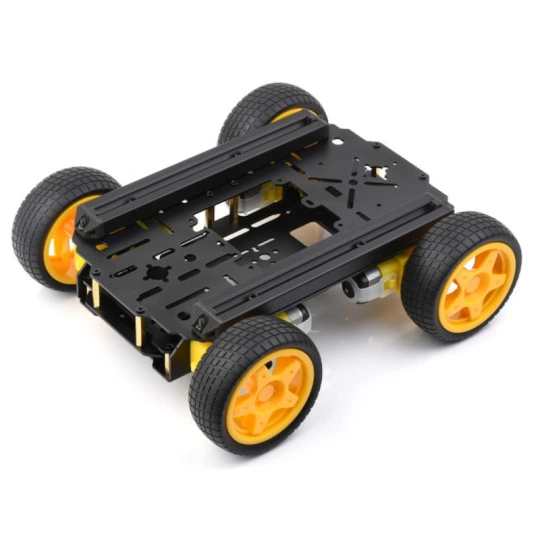
\includegraphics[width=0.7\textwidth]{chassis-waveshare-24419.png}
        \caption{Rama testowa Waveshare 24419}
        \label{fig:test_chassis}
    \end{figure}

    Rama wstępnie została przerobiona aby możliwe było sterowanie przednią osią. Zgodnie z zdjęciem \ref{fig:frontAxis_model}.
    Dodatkowo, został zmieniony sposób montażu silników, które zostały zamocowane na odwrotnie do zaleceń producenta, a także, zrezygnowano z ,,gumek", odpowiadających za amortyzację.


    % TODO: dodać opis ramy pojazdu

    \subsection{Pomiar odległości}
        Pomiar odległości jest podstawową funkcjonalności, współczesne pojazdy autonomiczne wykorzystują układy LIDAR, które pozwalają mierzyć pełne $360^\circ$.
        Jednak w wielu sytuacjach taki pomiar mija się z celem, gdyż znaczna większość próbek zostaje odrzucona.
        Same lidary, zaś są bardzo drogimi urządzeniami, często z niestandardowym sposobem komunikacji (np. za pomocą UART). 
        Dlatego, też autorzy, zdecydowali się na zastosowanie tańszych czujników ToF.
        Trzy takie czujniki zostały zamocowane z przodu pojazdu, z rozstawieniem co $30^\circ$.
        Na rysunku \ref{fig:ToF_holder}, przedstawiono wyżej opisany sposób montażu.
\newpage
        \begin{figure}[!ht]
            \centering
            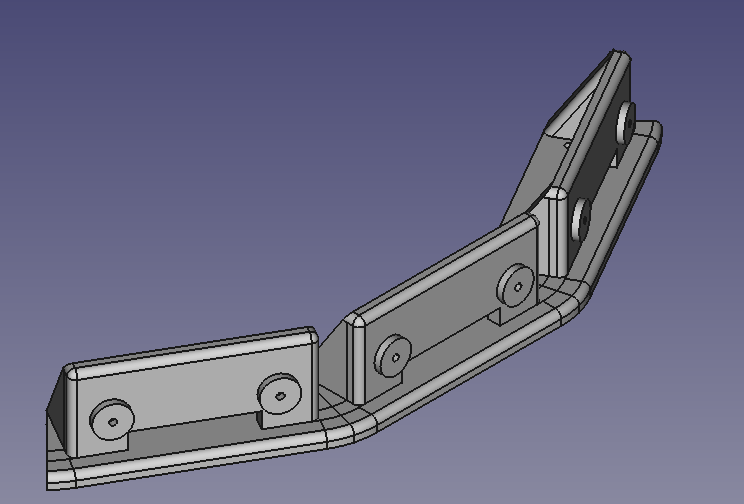
\includegraphics[width=0.7\textwidth]{ToF_holder.png}
            \caption{Mocowanie czujników ToF}
            \label{fig:ToF_holder}
        \end{figure}
